\documentclass[11pt]{beamer}
\usetheme{Copenhagen}

\defbeamertemplate*{headline}{split}
{%
  \leavevmode%
  \hbox{%
  \begin{beamercolorbox}[wd=.5\paperwidth,ht=2.65ex,dp=1.5ex,right]{section in head/foot}%
    \usebeamerfont{section in head/foot}\insertsectionhead\hspace*{2ex}
  \end{beamercolorbox}%
  \begin{beamercolorbox}[wd=.5\paperwidth,ht=2.65ex,dp=1.5ex,left]{subsection in head/foot}%
    \usebeamerfont{subsection in head/foot}\hspace*{2ex}\insertsubsectionhead
  \end{beamercolorbox}}%
  \vskip0pt%
}

\defbeamertemplate*{footline}{split}
{
	\leavevmode%
   	\hbox{%
      \begin{beamercolorbox}[wd=.5\paperwidth,ht=2.25ex,dp=1ex,center]{author in head/foot}%
        \usebeamerfont{author in head/foot}\insertshortauthor
      \end{beamercolorbox}%
      \begin{beamercolorbox}[wd=.4\paperwidth,ht=2.25ex,dp=1ex,center]{title in head/foot}%
        \usebeamerfont{title in head/foot}\insertshorttitle
      \end{beamercolorbox}%
      \begin{beamercolorbox}[wd=.1\paperwidth,ht=2.25ex,dp=1ex,right]{date in head/foot}%
        \usebeamerfont{date in head/foot}
        \insertframenumber{} / \inserttotalframenumber\hspace*{2ex}
      \end{beamercolorbox}}%
      \vskip0pt%
}

\setbeamertemplate{caption}{\raggedright\insertcaption\par}



\usepackage[utf8]{inputenc}
\usepackage{amsmath}
\usepackage{amsfonts}
\usepackage{amssymb}
\usepackage{graphicx}
\usepackage{lmodern}
\usepackage{multirow}
\graphicspath{ {./figures/} }
\author{Arthur Mensch, Michaël Weiss}
\title{Bandits on Stochastic Blockmodel Graphs}
%\setbeamercovered{transparent} 
\setbeamertemplate{navigation symbols}{} 
%\logo{} 
\institute{Reinforcement Learning} 
\date{January 2015} 
%\subject{}

\DeclareMathOperator*{\expect}{\mathbb{E}}

\AtBeginSection[]
{
  \begin{frame}
    \frametitle{Table of contents}
    \tableofcontents[currentsection]
  \end{frame}
}


\begin{document}

\begin{frame}
\titlepage
\end{frame}

\begin{frame}{Introduction}
\begin{columns}
	\begin{column}{.5\textwidth}
		\begin{figure}[ht]
			\centering
			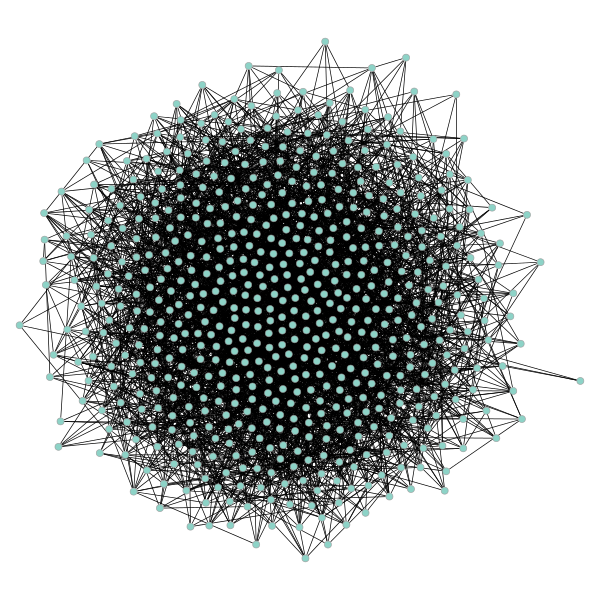
\includegraphics[width=.6\textwidth]{blockmodel3}
			\caption{Erdos Renyi Graph}
		\end{figure}
	\end{column}
	\begin{column}{.5\textwidth}
	\begin{figure}[ht]
		\centering
		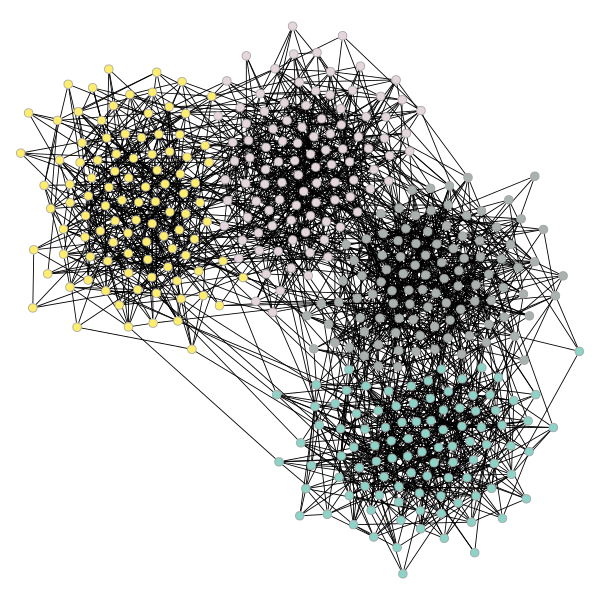
\includegraphics[width=.6\textwidth]{blockmodel1}
		\caption{Other random graph}
	\end{figure}
	\end{column}
\end{columns}
\begin{block}{Problem}
Multi arm bandit problem with side information to exploit
\end{block}
\end{frame}

\begin{frame}
\tableofcontents
\end{frame}
\section{\textsc{Exp3} on Erdös-Rényi Graph}
\begin{frame}{Problem definition}
$N$ arms, $T$ steps.
\begin{enumerate}
\item The environment chooses losses for every arm noted $l_{t,i}$ for the arm $i$ at the step $t$.
\item Following the algorithm we hope would minimize as much as possible the regret the player draws an arm $I_t$.
\item The player receives the loss $l_{t,I_t}$.
\item We define $\left(O_t\right)_{_i\in\left[N\right]}$ as the indicative function of observed loss at step $t$. We have:
\begin{align*}
O_{t,I_t}=1 \qquad \forall i \neq I_t,\, O_{t,i} \sim B\left(r\right.)
\end{align*}
$\left(O_t\right)_{_i\in\left[N\right]}$ corresponds to the value of the logic expression $ i \ is\ neighbor\ of\ I_t$ in the Erdös-Rényi random graph drawn at step t.
\item For all $i$ such that $O_{t,i}=1$ the player can observe the loss $l_{t,i}$.
\end{enumerate}
\end{frame}

\begin{frame}{Duplex tricks}
Ideally,
\[
\hat{l}_{t,i}=\frac{O_{t,i}l_{t,i}}{p_{t,i} + (1-p_{t,i})r}.
\]
\begin{block}{Definition geometrical random variables}
\begin{align*}
M_t^* &=\min\{1\leq i<N: O_{t-1,i}^{'} =1\}\cup\{N\}\\
G_{t,i}&=\min\left(K_{t,i},M_t\right)
\end{align*}
\end{block}
\begin{block}{Independence}
\begin{align*}
p_{t+2,i} \text{ estimated at the end of the step t.}
\end{align*}
\end{block}
So we can compute,
\begin{align*}
\hat{l}_{t,i}=G_{t,i}O_{t,i}l_{t,i}
\end{align*}
\end{frame}

\begin{frame}{Generalizing}
\textsc{Estimate\_r} gives a safe lower bounding on r.
\begin{align*}
&\text{If }\underline{r}=0,\ & \text{ we run vanilla } \textsc{Exp3}.\\
&\text{If } \underline{r} \geq \frac{\log T}{N},\  & \text{ we run vanilla }\textsc{Duplex}.\\
&\text{If } 0 < \underline{r} < \frac{\log T}{N},\ & A =\left\lceil \frac{\log T}{N \underline{r}} \right\rceil \text{and run } \textsc{Duplex} \text{ grouping } A \text{ steps}.  
\end{align*}
\end{frame}

\section{\textsc{Exp3} on Stochastic Block-Model Graphs}
\begin{frame}{Random graph with Stochastic Block-Model}
\begin{figure}[ht]
	\centering
	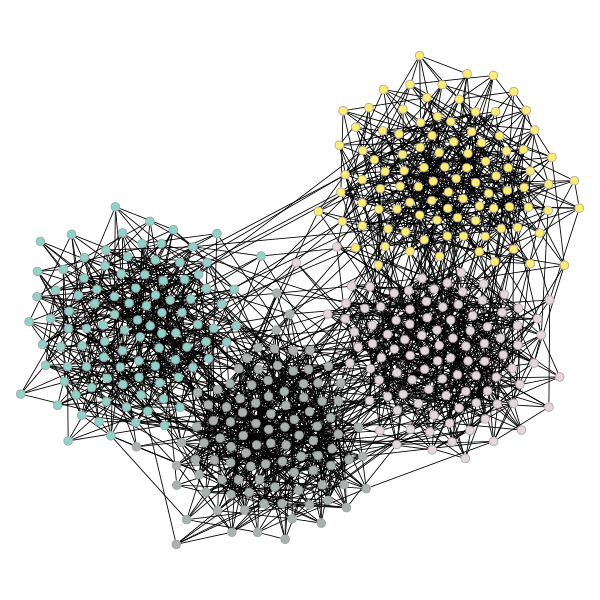
\includegraphics[width=.5\textwidth]{blockmodel_unsuccess}
	\caption{Neighbor communities}
\end{figure}
\end{frame}

\begin{frame}{Probability of side information}
\begin{itemize}
\item N clusters
\item Labeled vertices
\item $R=(r_{ij})_{1 \leq i,j \leq n} $ the matrix representing the probability of having side information.
\item $r_{ij}$ represents the probability that a vertex of the cluster $j$ reveals his loss to a given vertex of the cluster $i$
\end{itemize}

\end{frame}

\begin{frame}{Adapt $M_t$ sampling}
\begin{block}{Unbiased estimator}
\begin{align*}
\hat{l}_{t,i}^{*} = \frac{O_{t,i}l_{t,i}}{p_{t,i}+(1-p_{t,i})r_{C(I_t),C(i)}}
\end{align*}
\end{block}
\begin{block}{Using data...}
\begin{align}
\hat{l}_{t,i}=G_{t,i}O_{t,i}l_{t,i}
\end{align}
\begin{itemize}
\item Estimator $G_{i,t} \sim G(p_{t,i}+(1-p_{t,i})r_{I_t,i})$
\item $M_t^i$ truncated geometric law of parameter $p_{t,i}$
\item[$\rightarrow$] $G_{t,i}=\min\left(K_{t,i},M_t^i\right)$
\end{itemize}
\end{block}
\end{frame}

\begin{frame}{Sampling $M_t^i$}

\begin{block}{Algorithm adaptation}
\begin{itemize}
\item Using previous observations
\item Ensure independence of $M_t$ and $O_t$
\item Find the last $O_{t'}$, with $t' \equiv t -1 [2]$ in which $C(I(t')) = C(I(t))$
\item Average the distance between two observation within cluster $C(j)$.
\end{itemize}
\end{block}

\alert{Keeping track of last time we picked $I$ in cluster $i$}

\end{frame}


\begin{frame}{Lower bounding R}
\begin{itemize}
\item We adapt \textsc{Estimate\_r} so that it returns $\underline{R}$ where $\underline{r}_{ij} \leq r_{ij}$ with high probability.
\item This is done at the relatively low cost $\expect\left({\tau}\right) \leq \sum_{i,j \in [N]^2} \frac{4\log T}{N_i} \mathbf{1}_{r_{ij} > \frac{1}{N_j}} + \sqrt{T} \mathbf{1}_{r_{ij} < \frac{1}{N_j}}+ \mathrm{Cste}$
\end{itemize}
\end{frame}

\begin{frame}{Generalized algorithm with stochastic blockmodel graphs}
\begin{align*}
&\text{If }\underline{R}=0,\ & \text{ we run vanilla } \textsc{Exp3}.\\
&\text{If } \min_{i,j,\ \underline{r}_{i,j}>0} \left(\underline{r}_{ij}\: N_j \right) \geq \log T ,\  & \text{ we run adapted }\textsc{Duplex}. \\
&\text{Else},\ & A =\left\lceil \frac{\log T}{r_N*} \right\rceil \text{ where }\\
& & r_N*=\min_{i,j,\ \underline{r}_{i,j}>0} \left(\underline{r}_{ij}\: N_j \right) \\
& & \text{ and run } \textsc{Duplex} \text{ grouping } A \text{ steps}.  
\end{align*}
\end{frame}

\section{Results}


\begin{frame}{Test graphs}
\vspace{-1em}
\begin{columns}
	\begin{column}{.5\textwidth}
		\begin{figure}[ht]
			\centering
			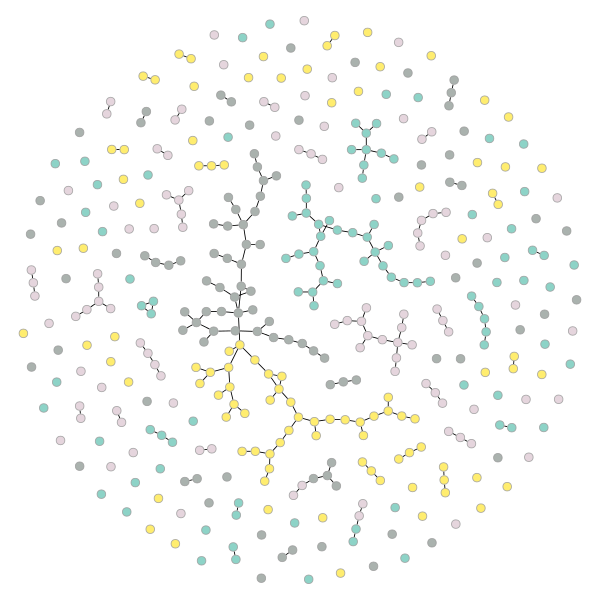
\includegraphics[width=.5\textwidth]{blockmodel0}
			\caption{Weakly assossiative}
		\end{figure}
		\vspace{-2em}
		\begin{figure}[ht]
			\centering
			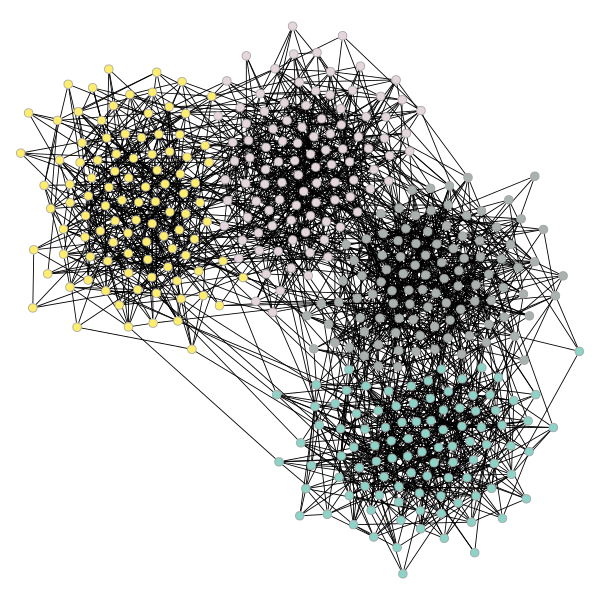
\includegraphics[width=.5\textwidth]{blockmodel1}
			\caption{Neighbours}
		\end{figure}
	\end{column}
	\begin{column}{.5\textwidth}
		\begin{figure}[ht]
			\centering
			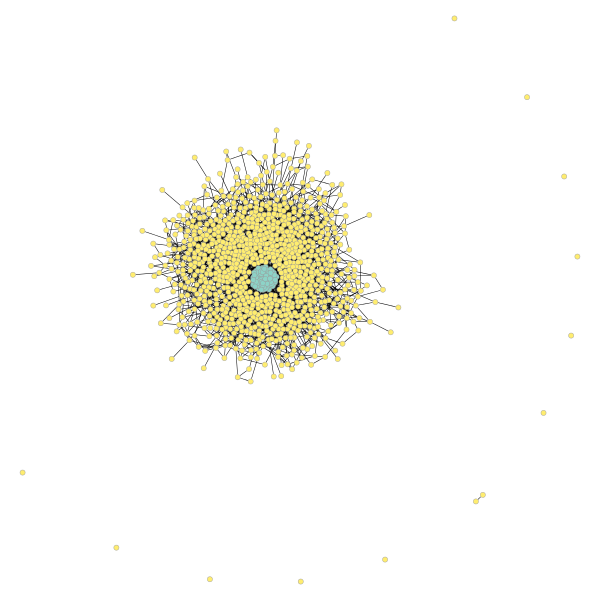
\includegraphics[width=.5\textwidth]{blockmodel2}
			\caption{Unbalanced}
		\end{figure}
		\vspace{-2em}
		\begin{figure}[ht]
			\centering
			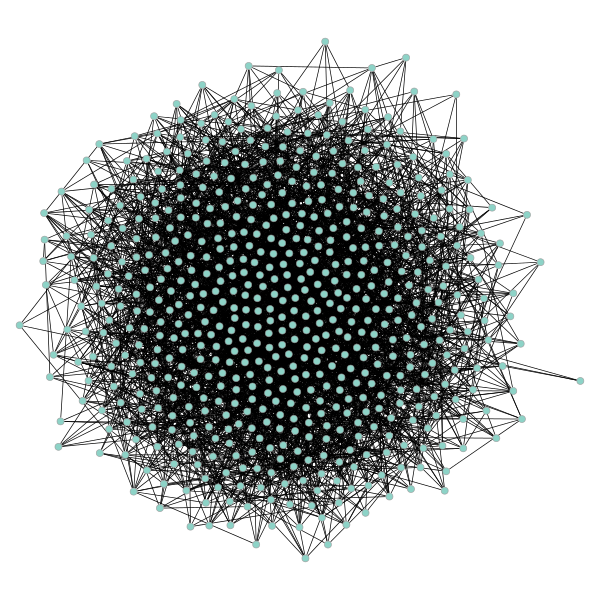
\includegraphics[width=.5\textwidth]{blockmodel3}
			\caption{Erdos-Rényi}
		\end{figure}
	\end{column}
\end{columns}
\end{frame}

\begin{frame}{Unbalanced}
\begin{figure}[ht]
	\centering
	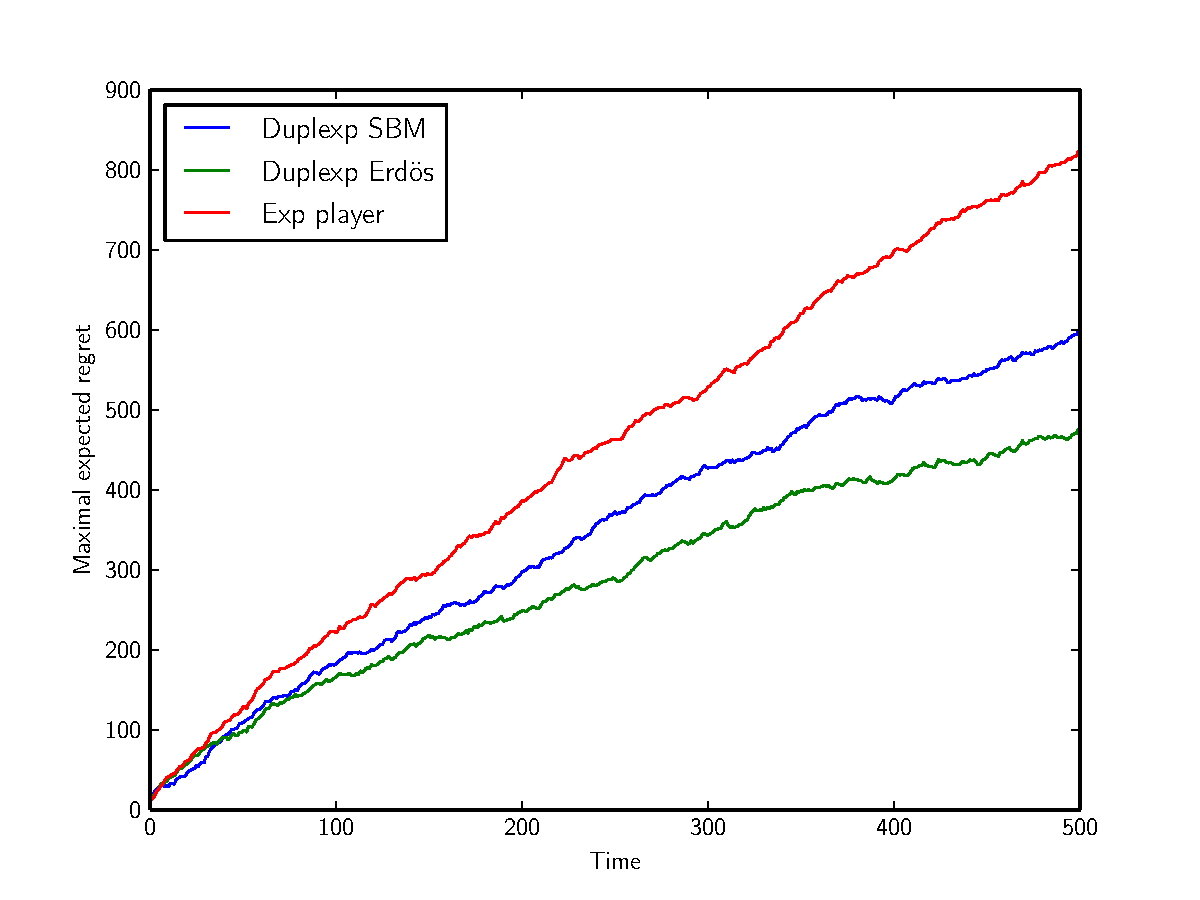
\includegraphics[width=.8\textwidth]{easy}
	\caption{Easy problem}
\end{figure}
\end{frame}

\begin{frame}{Unbalanced}
\begin{figure}[ht]
	\centering
	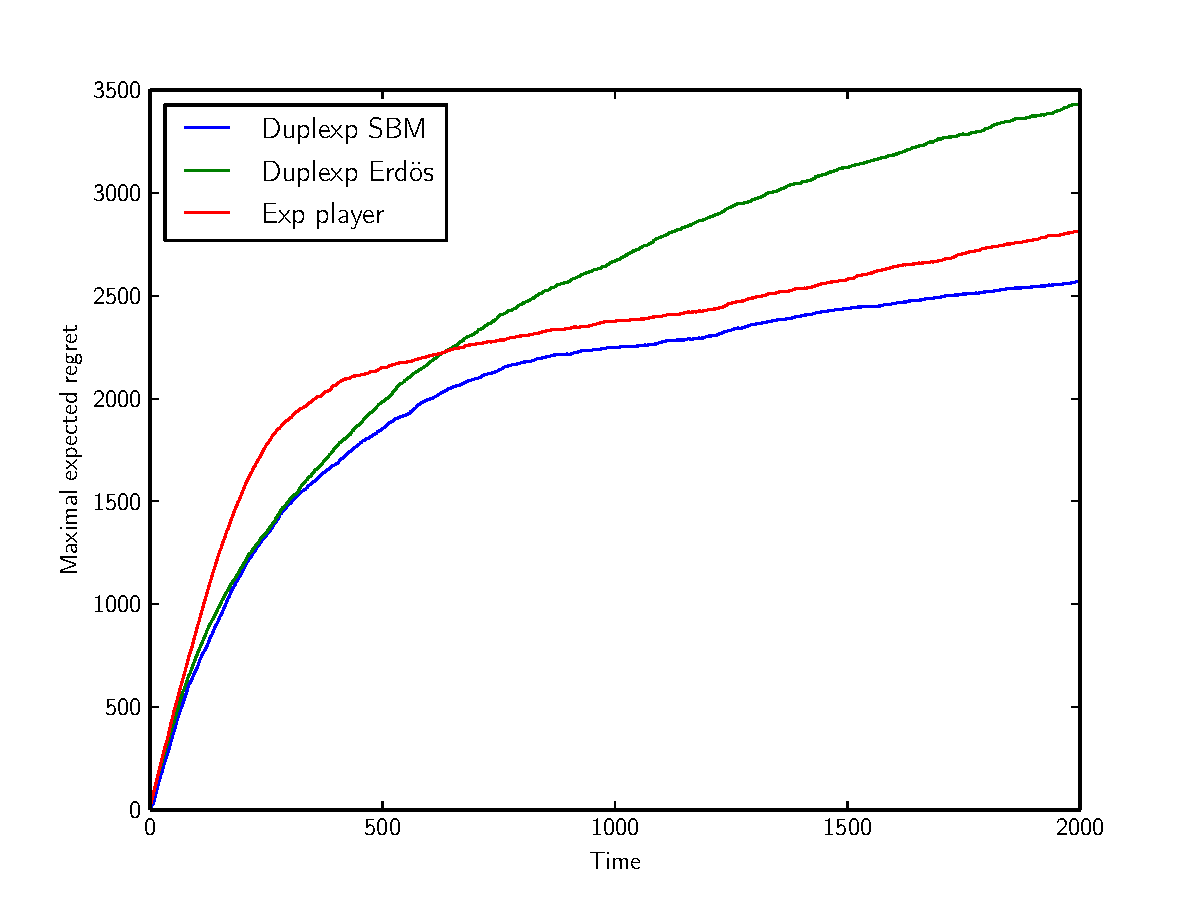
\includegraphics[width=.8\textwidth]{hard}
	\caption{Hard problem}
\end{figure}
\end{frame}

\begin{frame}{Neighbours}
\begin{figure}[ht]
	\centering
	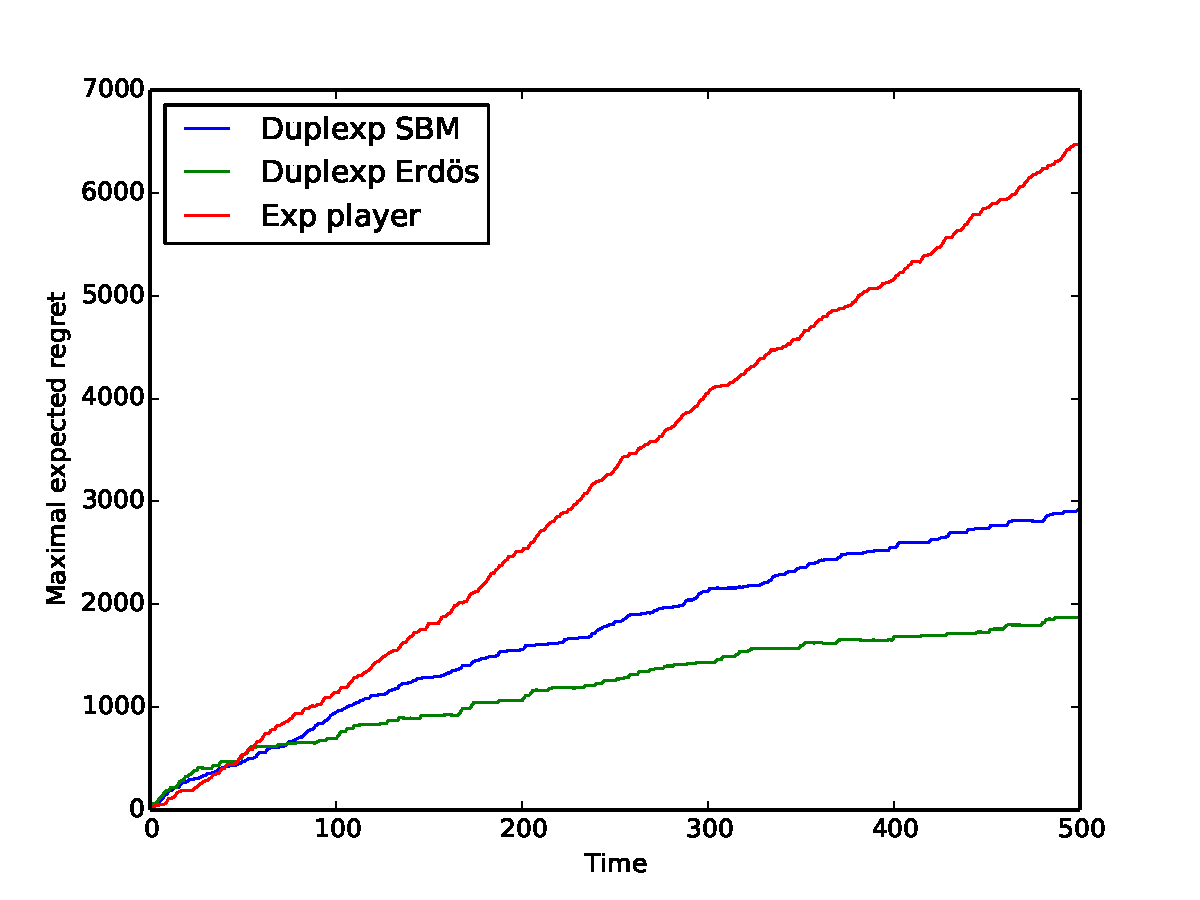
\includegraphics[width=0.8\textwidth]{regret_balanced_easy}
	\caption{Easy problem}
	\label{fig:easy}
\end{figure}
\end{frame}

\begin{frame}{Neighbours}
\begin{figure}[ht]
	\centering
	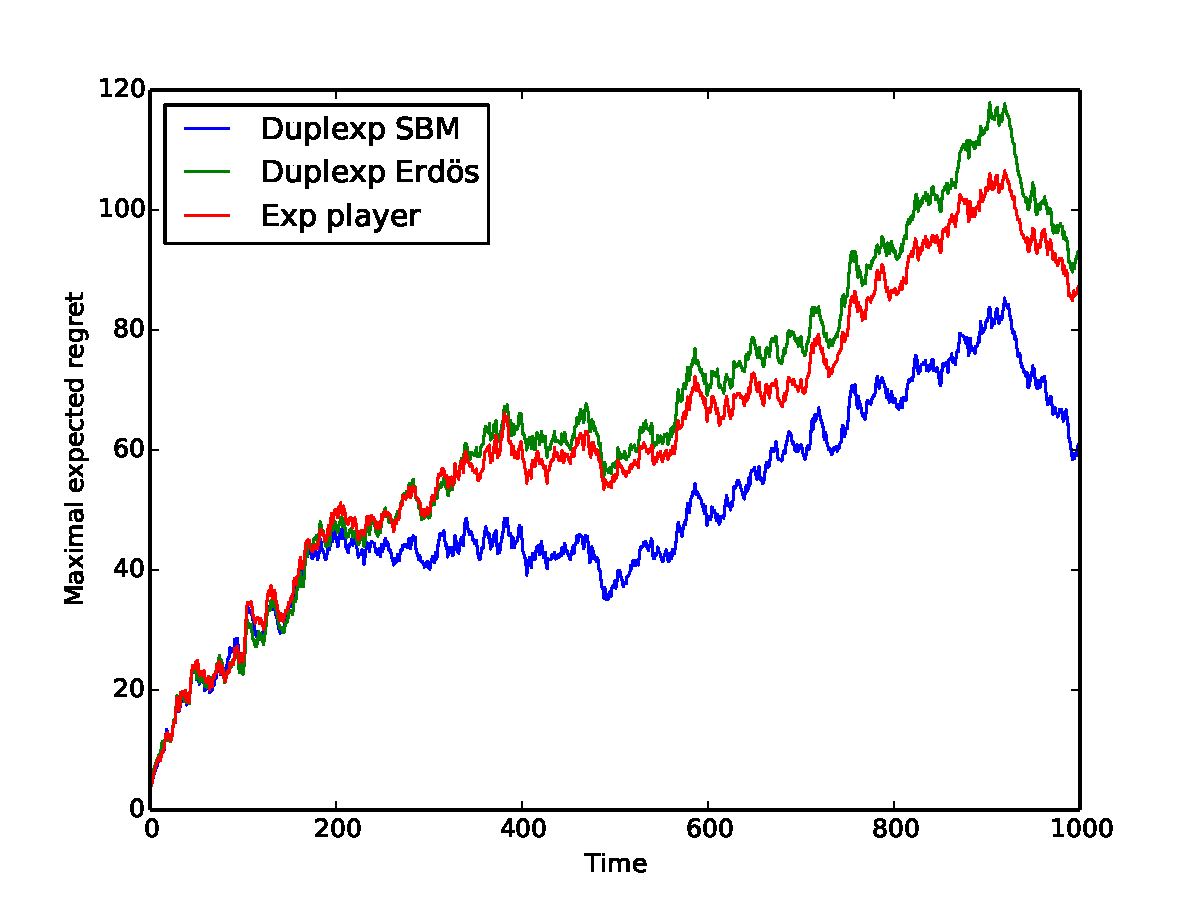
\includegraphics[width=0.8\textwidth]{regret_balanced_hard}
	\caption{Hard problem}
	\label{fig:easy}
\end{figure}
\end{frame}



\end{document}